\documentclass{article}
\usepackage{graphicx} % Required for inserting images

\title{Florida}
\author{Harry Trevelyan}
\date{}

%% Page size and margins
\usepackage[a4paper,top=2.1cm,bottom=2.1cm,left=3cm,right=3cm,marginparwidth=1.75cm]{geometry}

%% Useful packages
\usepackage{amsmath}
\usepackage{graphicx}
\usepackage[colorinlistoftodos]{todonotes}
\usepackage[colorlinks=true, allcolors=blue]{hyperref}
\usepackage{float} % Control the position of figures
\usepackage[font=small, labelfont=bf]{caption} % Set figure caption style
\usepackage{setspace} % For line spacing
\setstretch{1} % Set default line spacing to 1.2

\title{Is Florida Warming? A Permutation Analysis of Florida Temperature Data}
\author{Harry Trevelyan}
\date{} % Remove the date

\setlength{\textfloatsep}{4pt}
\setlength{\belowcaptionskip}{4pt}


\begin{document}

\maketitle

\section*{Methods}
To assess whether there was a statistically significant correlation between temperature and year, a permutation analysis was conducted. First, the Pearson correlation coefficient between year and temperature was calculated for the observed data. This procedure was repeated on 10,000 duplicate time series, in which the temperature values were randomly shuffled, to generate a distribution of correlation coefficients under the null hypothesis of no correlation (Figure 1B). The p-value for our observed correlation was estimated as the proportion of permuted correlations that were greater than or equal to the observed correlation.

\section*{Results and Discussion}
Temperature data were recorded over a 100-year period (1901-2000). The mean temperature was 21.31°C (SD = 0.50°C). 

The observed Pearson correlation coefficient between temperature and year was calculated as 0.56, indicating a moderate positive correlation which is evident in a simple scatter plot (Figure 1A). In none of the permuted time series did we calculate a correlation coefficient of this magnitude (Figure 1B), so the p-value was estimated to be less than 0.001. This suggests that the relationship between temperature and year is statistically significant, allowing us to confidently reject the null hypothesis of no correlation.


\begin{figure}[ht]
    \centering
    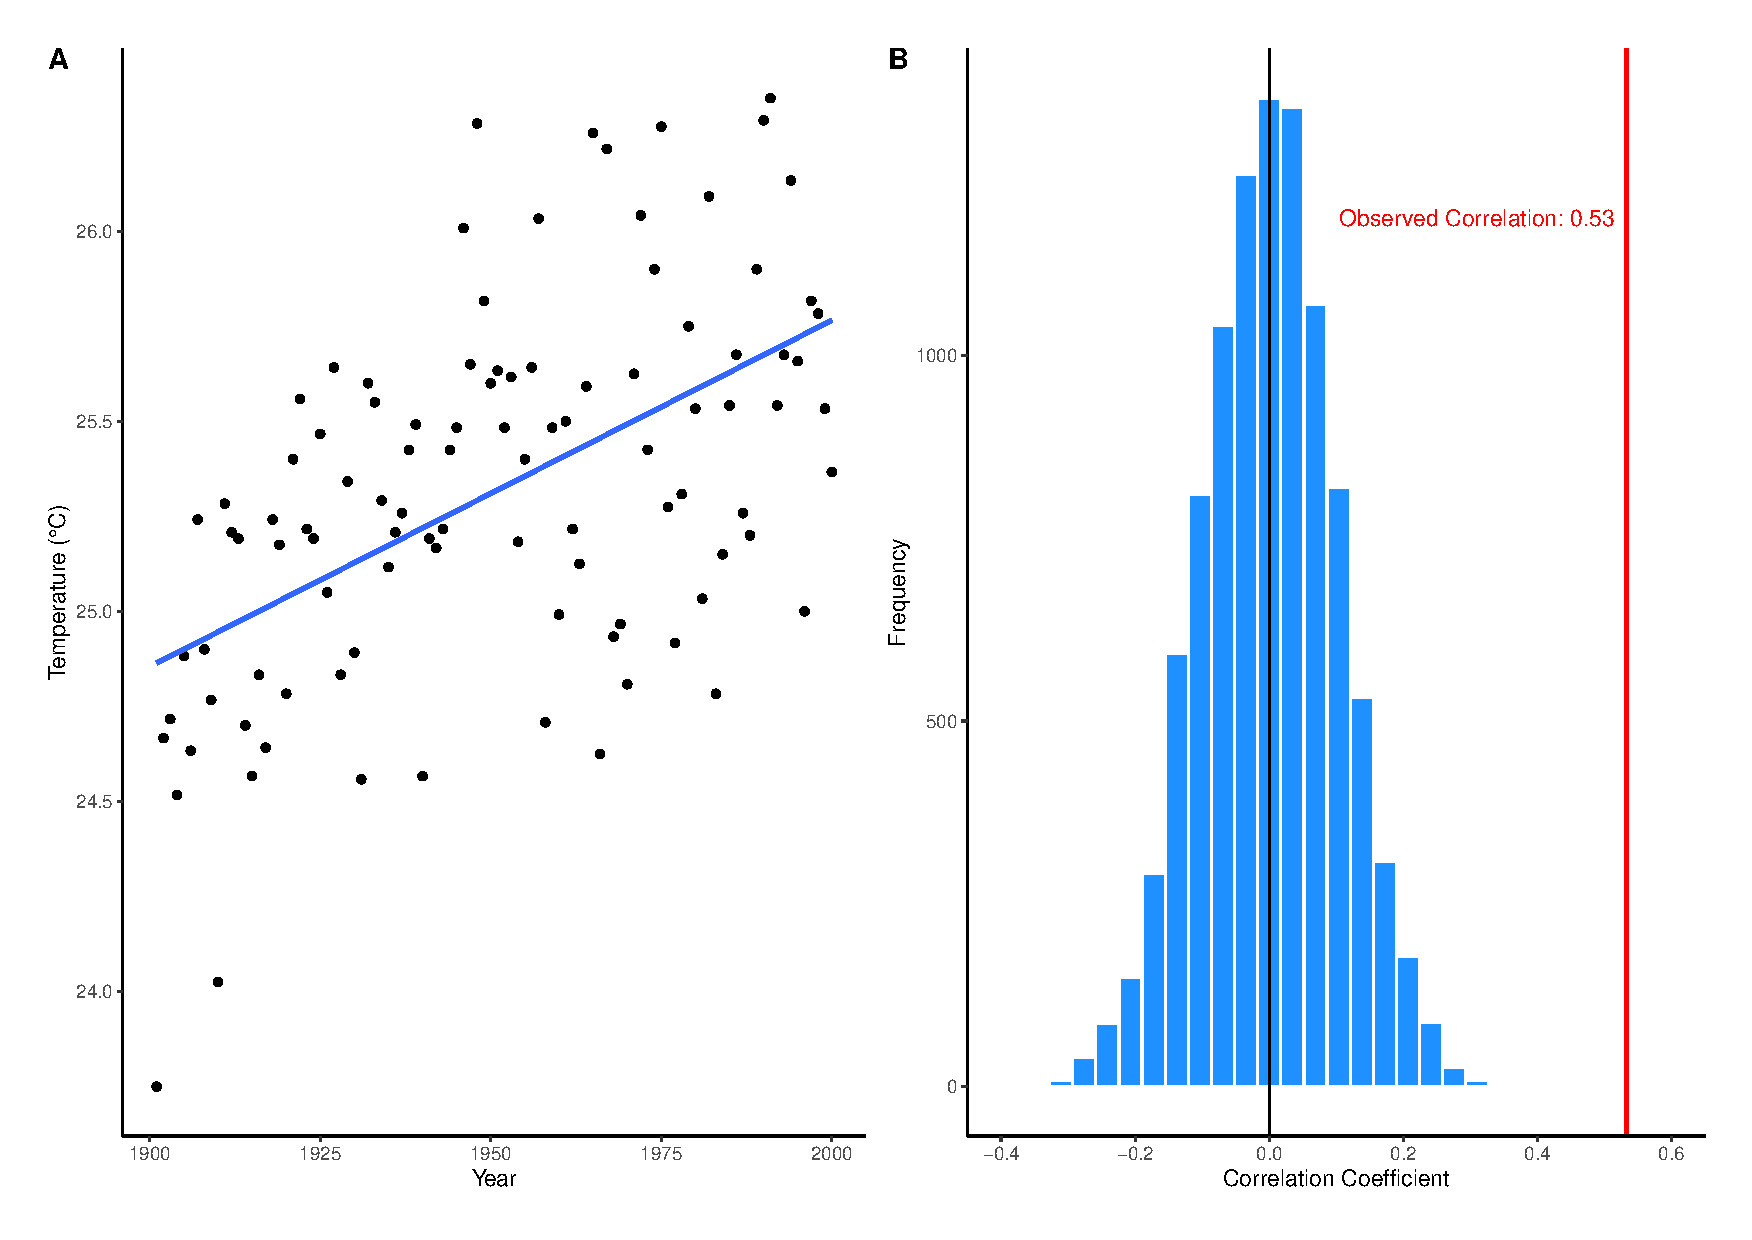
\includegraphics[height = 0.6\textwidth]{../results/Florida_plots.pdf}
    \caption{ A) Correlation between year and temperature from 1901-2000 in Florida. Confidence intervals are not displayed around the regression line due to potential autocorrelation within the data. B) Randomized correlation coefficient distribution. The histogram displays the distribution of correlation coefficients from 10,000 randomly permuted time series. The red line indicates the observed correlation coefficient. }
    \label{fig:floridaplots}
\end{figure}


\end{document}
